\begin{table}[t!]
    \begin{minipage}[t!]{\textwidth}
      \begin{minipage}[b]{0.5\textwidth}
        \centering 
            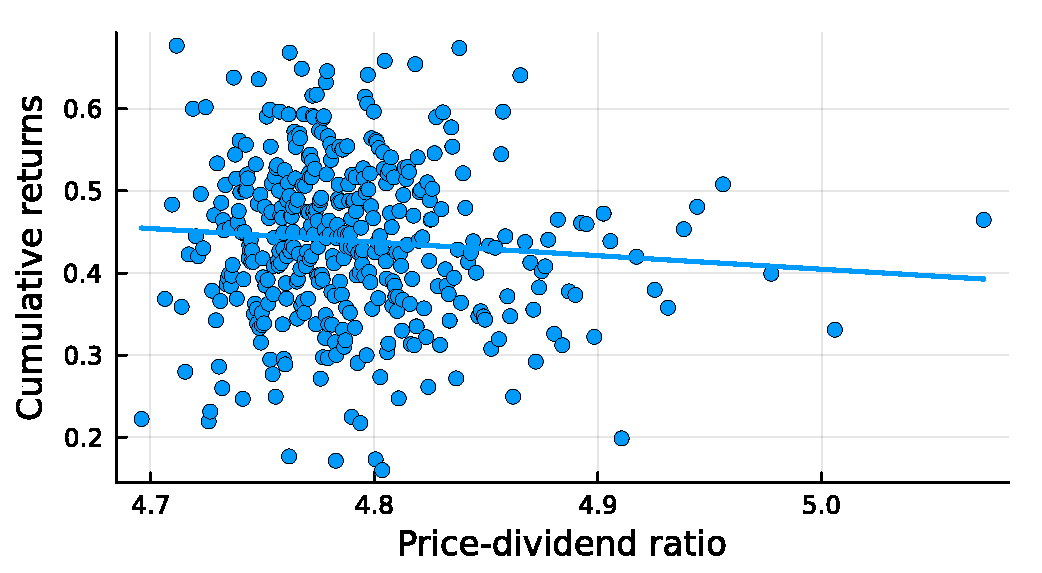
\includegraphics[width=0.99\textwidth]{figures/pd_forecast_binscatter.pdf}
        \captionof{figure}{Return predictability}\label{fig:pd_scatter}
        \end{minipage}
        \hfill
      \begin{minipage}[b]{0.5\textwidth}
        \centering
            \scriptsize
    \begingroup
    \centering\scalebox{0.99}{
    \begin{tabular}{lcccc}
       \tabularnewline \midrule \midrule
       Dependent Variable: & \multicolumn{4}{c}{cum\_ex\_returns}\\
       Model:         & (1)           & (2)            & (3)            & (4)\\  
       \midrule
       \emph{Variables}\\
       labor\_income    &   -2.07   &           & 0.33      &           \\   
                        &   (0.94)  &           & (1.31)    &           \\
       p/d              &           & -0.29     &           & -0.04     \\   
                        &           & (0.12)    &           & (0.17)    \\   
       \midrule
       Observations   & 4,000           & 4,000            & 4,000            & 4,000\\  
       \midrule \midrule
       %\multicolumn{5}{l}{\emph{Heteroskedasticity-robust standard-errors in parentheses}}\\
       \multicolumn{5}{l}{\emph{\textcolor{white}{Signif. Codes: ***: 0.01, **: 0.05, *: 0.1}}}\\
    \end{tabular}}
    \par\endgroup
          \captionof{table}{Labor and p/d ratio regressions}\label{table:pred_regression}
      \end{minipage}
      
      \end{minipage}    
          \caption*{\scriptsize 
        Note: The left panel shows a binscatter plot based on model simulations of the price-dividend ratio and a measure of future cumulative returns, $\sum_{k=1}^T \rho^{k-1} r_{t+k}$, for $T = 60$ quarters. We sort the first 4,000 observations by the price-dividend ratio into 400 equal-count bins and plot bin averages. The right panel shows the regression coefficients of future cumulative excess returns for $T = 60$ on the price-dividend ratio and labor income. 
        The data for the first two columns was simulated under the objective measure, while the data for the last two columns was simulated under subjective beliefs. Entries report Monte Carlo mean coefficients, and parentheses report the standard deviation across simulations.
         }
    \end{table}
